\documentclass{beamer}
\usepackage[utf8]{inputenc}

\usetheme{Madrid}
\usecolortheme{default}
\usepackage{amsmath,amssymb,amsfonts,amsthm}
\usepackage{txfonts}
\usepackage{tkz-euclide}
\usepackage{listings}
\usepackage{adjustbox}
\usepackage{array}
\usepackage{tabularx}
\usepackage{gvv}
\usepackage{lmodern}
\usepackage{circuitikz}
\usepackage{tikz}
\usepackage{graphicx}

\setbeamertemplate{page number in head/foot}[totalframenumber]

\usepackage{tcolorbox}
\tcbuselibrary{minted,breakable,xparse,skins}



\definecolor{bg}{gray}{0.95}
\DeclareTCBListing{mintedbox}{O{}m!O{}}{%
  breakable=true,
  listing engine=minted,
  listing only,
  minted language=#2,
  minted style=default,
  minted options={%
    linenos,
    gobble=0,
    breaklines=true,
    breakafter=,,
    fontsize=\small,
    numbersep=8pt,
    #1},
  boxsep=0pt,
  left skip=0pt,
  right skip=0pt,
  left=25pt,
  right=0pt,
  top=3pt,
  bottom=3pt,
  arc=5pt,
  leftrule=0pt,
  rightrule=0pt,
  bottomrule=2pt,
  toprule=2pt,
  colback=bg,
  colframe=orange!70,
  enhanced,
  overlay={%
    \begin{tcbclipinterior}
    \fill[orange!20!white] (frame.south west) rectangle ([xshift=20pt]frame.north west);
    \end{tcbclipinterior}},
  #3,
}
\lstset{
    language=C,
    basicstyle=\ttfamily\small,
    keywordstyle=\color{blue},
    stringstyle=\color{orange},
    commentstyle=\color{green!60!black},
    numbers=left,
    numberstyle=\tiny\color{gray},
    breaklines=true,
    showstringspaces=false,
}
\begin{document}

\title 
{5.8.4}
\date{September 28,2025}


\author 
{ADUDOTLA SRIVIDYA -EE25BTECH11006}






\frame{\titlepage}

\begin{frame}{Question}
Half the perimeter of a rectangular garden, whose length is 4m more than its width, is 36m. Find the dimensions of the garden.
\end{frame}

\begin{frame}{Formulating the Equations}
Let length be l, breadth be b.

\begin{align}
\text{Half perimeter:} \quad & l + b = 18 \\
\text{Length exceeds breadth by 4m:} \quad & l - b = 4
\end{align}

Matrix form:
\begin{align}
\myvec{1 & 1 \\ 1 & -1} \myvec{l \\ b} = \myvec{18 \\ 4}
\end{align}
\end{frame}

\begin{frame}{Solving Using Orthogonal Matrix}
Let
\begin{align}
    \vec{A} = \myvec{1 & 1 \\ 1 & -1}, \quad \vec{X} = \myvec{l \\ b}, \quad \vec{Y} = \myvec{18 \\ 4}
\end{align}
\begin{align}
    \vec{A}^T \vec{A} = \myvec{1 & 1 \\ 1 & -1}^T \myvec{1 & 1 \\ 1 & -1} 
          = \myvec{2 & 0 \\ 0 & 2} = 2I
\end{align}
Since $\vec{A}^T \vec{A} = 2I$, we have
\begin{align}
    \vec{A}^{-1} = \dfrac{1}{2}\vec{A}^T
\end{align}
\end{frame}

\begin{frame}{Solving Using Orthogonal Matrix}
\begin{align}
\vec{X}&= \vec{A}^{-1}\vec{Y} \\
       &= \frac{1}{2}\vec{A}^T \vec{Y} \\
       &= \frac{1}{2}\myvec{1 & 1 \\ 1 & -1}\myvec{18 \\ 4} \\
       &= \frac{1}{2}\myvec{22 \\ 14} \\
       &= \myvec{11 \\ 7}
\end{align}
\end{frame}

\begin{frame}{Final Answer}
Solution:
\begin{align}
\vec{X} = \myvec{11 \\ 7}
\end{align}

\textbf{Therefore:}
\begin{align}
 Length = 11m \ \ \ \ \ 
 Breadth = 7m
\end{align}
\end{frame}

\begin{frame}[fragile]
\frametitle{Python,C,Python+C codes}
codes permalink
\end{frame}

\begin{frame}{Plot}
    \centering
    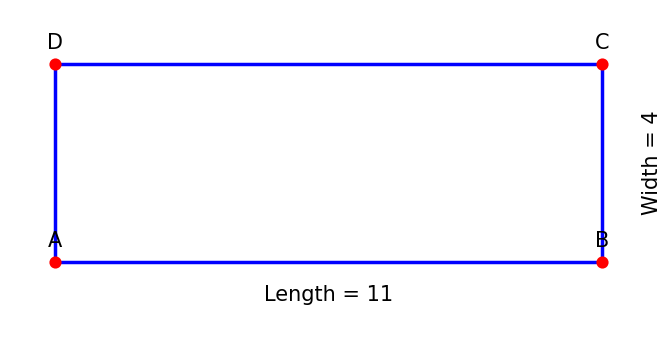
\includegraphics[width=\columnwidth, height=0.8\textheight, keepaspectratio]{figs/fig.png}
\end{frame}

\end{document}